\section{Desenvolvimento do Projeto}

\subsection{Repositório do Código Fonte do Projeto}

O código está disponível em \url{https://github.com/ReadRace-AGES/ReadRace}. O projeto utiliza um monorepositório com as pastas \texttt{backend} e \texttt{mobile}, tendo \texttt{dev} como branch principal de desenvolvimento. As tarefas são acompanhadas em \url{https://github.com/orgs/ReadRace-AGES/projects/1}. A wiki institucional reúne escopo, configuração e arquitetura: \url{https://tools.ages.pucrs.br/2026-2/6lmnp/readrace/readrace-wiki/-/wikis/home}.

Além do código, o repositório de gestão AGESIV reúne requisitos, decisões de produto, planejamento, épicos, dependências e fontes de referência. Nele estão documentadas 37 tarefas planejadas para a primeira sprint, organizadas em sete épicos. Há automações de apoio à elaboração de tarefas com IA e à publicação de issues. Esse material permite relacionar cada tarefa ao requisito, ao protótipo e às regras de negócio, mas não substitui a validação das decisões nem o acompanhamento das pessoas.

\subsection{Banco de Dados Utilizado}

O sistema utiliza PostgreSQL 16, com alterações estruturais versionadas por migrations do Flyway. O Hibernate valida o schema, enquanto as migrations são responsáveis por sua evolução. O modelo relacional em DBML, versão 8, contempla usuários, livros, autores, gêneros, itens da biblioteca e registros de leitura, além de entidades sociais e de gamificação.

Entre os relacionamentos estão os vínculos entre livros e autores, a associação dos livros à biblioteca de cada usuário, a participação em clubes e comunidades, os desafios entre amigos e as conquistas. A presença dessas entidades no modelo não significa que todas as funcionalidades tenham sido entregues: parte delas sustenta evoluções previstas para as próximas sprints.

A revisão da coerência entre esse modelo e as user stories foi uma das minhas contribuições. Em agosto, identifiquei divergências, registrei dúvidas e discuti sugestões com os demais AGES IV para alinhamento com os colegas responsáveis pela modelagem.

\subsection{Arquitetura Utilizada}

O aplicativo mobile comunica-se com uma API Spring Boot, que concentra as regras de negócio e o acesso ao PostgreSQL. O backend organiza suas responsabilidades em Controller, Service e Repository. Para a consulta ao catálogo externo de livros, a documentação descreve uma interface com adaptadores: uma base local atende desenvolvimento e testes, enquanto a integração com Google Books é selecionada em produção.

No mobile, o expo-router organiza as rotas e as telas são agrupadas por funcionalidades. O tema e os componentes compartilhados favorecem a consistência da interface. Durante a Sprint 1, a identificação do usuário foi simplificada por meio de um usuário fixo dos dados iniciais, resolvido pelo backend; a autenticação completa não deve ser confundida com uma entrega dessa etapa.

\begin{figure}[H]
\centering
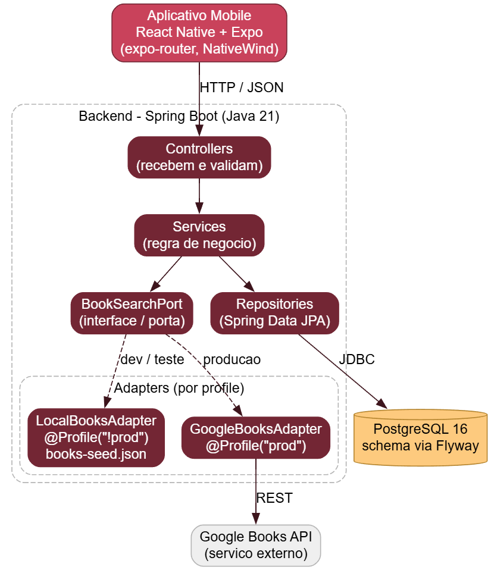
\includegraphics[width=\linewidth,height=0.42\textheight,keepaspectratio]{conteudo/5 - ages IV/conteudo/figures/arquitetura.png}
\caption{Arquitetura de aplicação do ReadRace.}
\legend{Fonte: wiki do projeto ReadRace.}
\end{figure}

A wiki descreve ainda uma arquitetura de implantação com Docker, NGINX, Cloudflare e serviços AWS, incluindo EC2, ECR e SSM Parameter Store. O uso de S3 aparece como previsto. Essa descrição registra a arquitetura documentada, sem representar uma validação independente do ambiente de produção.

\subsection{Protótipos das Telas Desenvolvidas}

Os protótipos foram elaborados no Figma: \url{https://www.figma.com/design/N5iThb17TAP2AOIZWBt2zK/ReadRace}. O planejamento da primeira sprint contemplou biblioteca, detalhe do livro, registro de progresso, comunidades, clubes, fórum, busca, perfil público e desafios entre amigos. As telas de desafios permaneceram pendentes ao final da sprint.

\begin{figure}[H]
\centering
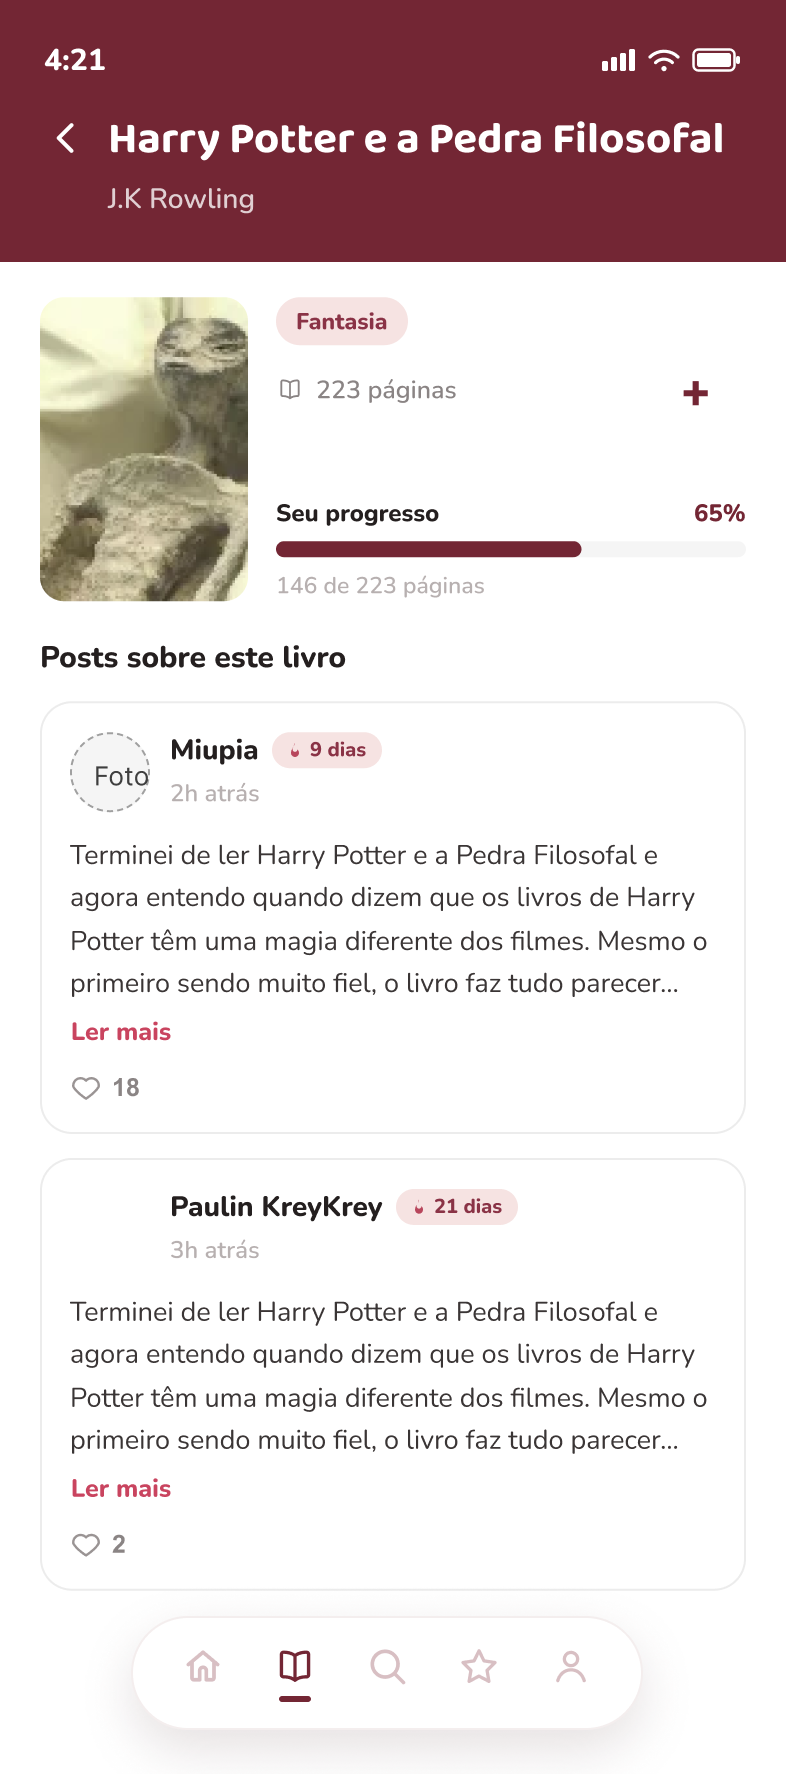
\includegraphics[width=0.43\linewidth,height=0.45\textheight,keepaspectratio]{conteudo/5 - ages IV/conteudo/figures/detalhe-livro.png}
\hspace{1cm}
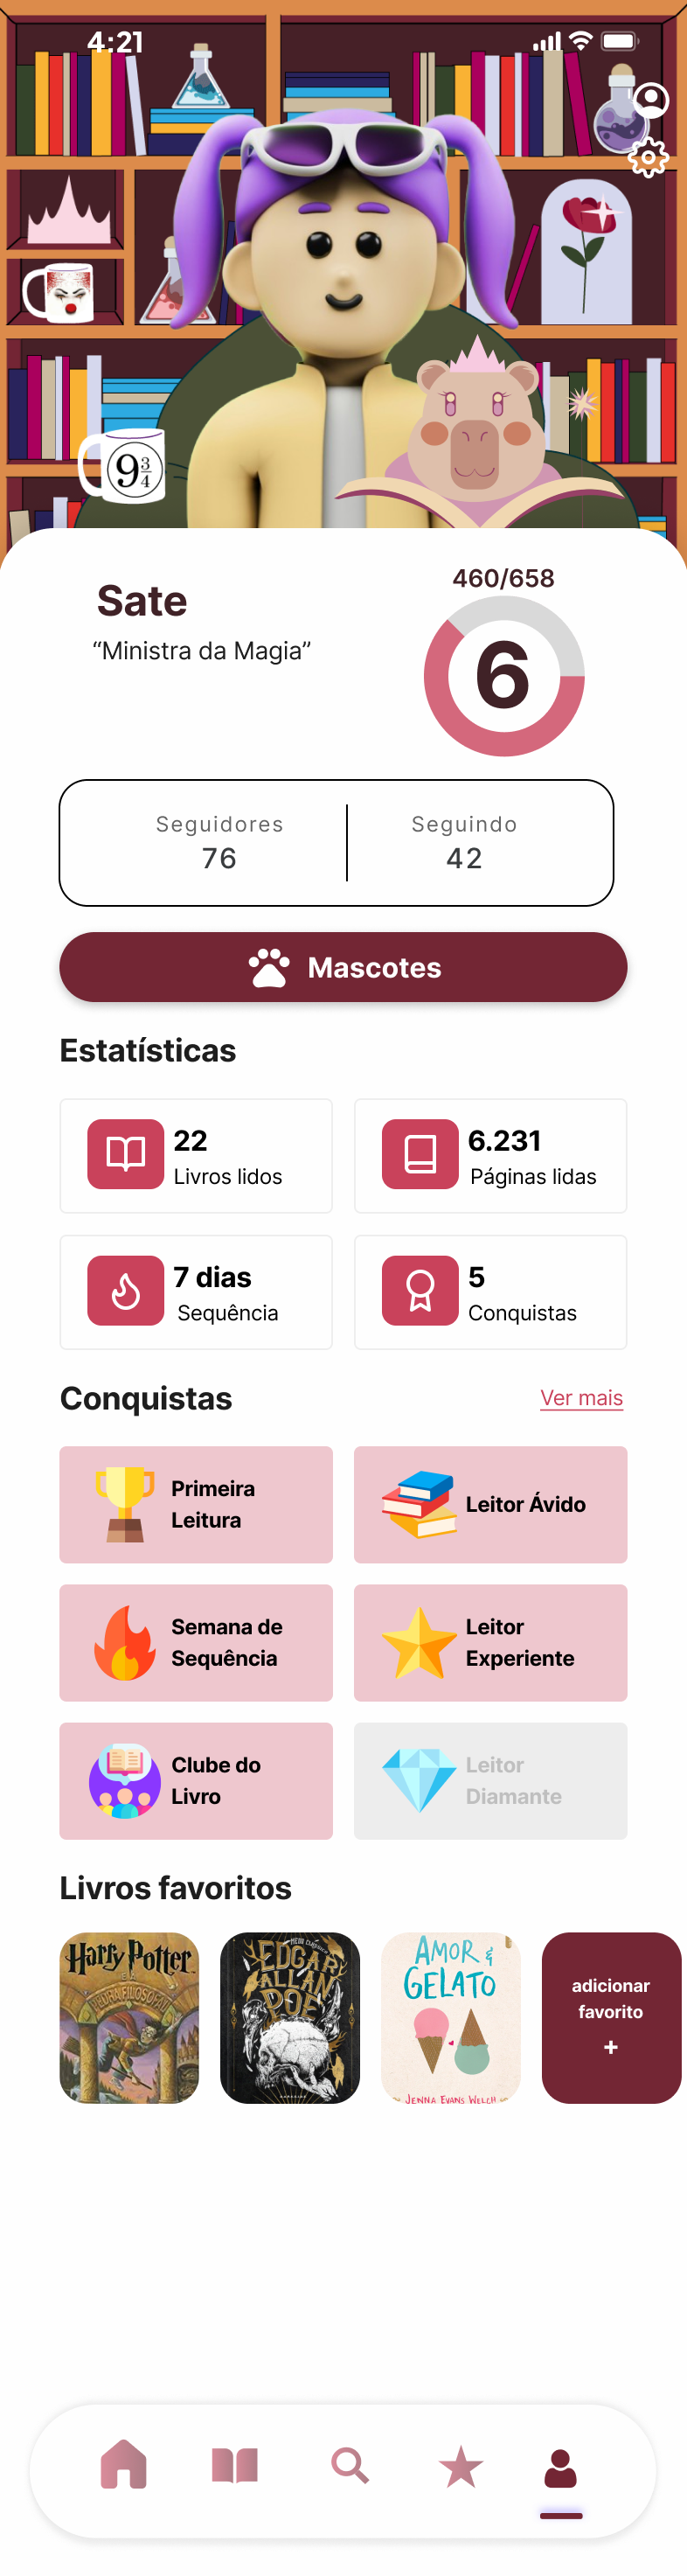
\includegraphics[width=0.43\linewidth,height=0.45\textheight,keepaspectratio]{conteudo/5 - ages IV/conteudo/figures/perfil.png}
\caption{Protótipos do detalhe do livro e do perfil do usuário.}
\legend{Fonte: exportações do Figma mantidas no repositório AGESIV.}
\end{figure}

Essas imagens representam referências de design, não capturas da aplicação entregue. As user stories também registram diferenças entre os protótipos e o recorte da sprint, como ações ainda indisponíveis e elementos do perfil reservados para etapas posteriores.

\subsection{Tecnologias Utilizadas}

O mobile utiliza React Native, Expo, TypeScript, expo-router e NativeWind. O backend utiliza Java 21, Spring Boot, Spring Data JPA, Maven e Springdoc OpenAPI para documentação dos endpoints. A persistência utiliza PostgreSQL e Flyway. Docker e Docker Compose apoiam a execução local, e GitHub Actions executa verificações automatizadas.

O backend conta com testes unitários e de integração, incluindo Testcontainers, além de JaCoCo para cobertura e Spotless para formatação. No mobile, há verificações de tipos e testes de componentes. Essas ferramentas apoiam a revisão das entregas, mas não dispensam a validação dos fluxos no aplicativo. As configurações e convenções estão documentadas no README do repositório de código.
